\chapter{Implementation}

\section{Simulation}\label{sec:sim}
%Pr 1 St 2
\textsc{MeqSilhouette} is an observation and signal corruption simulator written in \textsc{Python} and {\sc MeqTrees} using the  {\sc measurement set}\footnote{https://casa.nrao.edu/Memos/229.html}  data format. A flow diagram of the simulator is shown in Fig.~\ref{flow}. Input to the simulator is a sky model and configuration file. The former is typically a time-ordered list of {\sc fits} images, where each image represents the source total intensity\footnote{Later versions of {\sc MeqSilhouette} will enable the full Stokes cubes as input.} over a time interval $\Delta t_{\rm src} = t_{\rm obs}/N_{\rm src}$, where $t_{\rm obs}$ is the observation length and $N_{\rm src}$ is the number of source images. The configuration file specifies all parameters needed by the pipeline to determine the particular observation configuration (array, frequency, bandwidth, start time, etc) and which signal corruption implementation should be employed. The primary outputs of the pipeline are an interferometric dataset in {\sc measurement set} format along with the closure phases and uncertainties and a dirty and/or cleaned image. The modular structure of the pipeline allows for multiple imaging and deconvolution algorithms to be employed.  The rest of this section is devoted to describing the implementation of each signal corruption module.

This section details the software architechure used for the simulation code as well as the RODRIGUES online interface. It will refer back to the signal corruption and simulation theory sections as well as the code itself. Futhermore the code has been written with the intention of being readable, hence minimum comments needed. This has hopefully been achieved through keeping to the logical flow underlying the code and explanatory names .  The highest level or driver script is written in Python which interfaces easily with other systems.  The bulk of the computational load is called through other programs, written in C++ which are faster. The CASA Measurement Set(MS) is data format of choice, although in the mm-VLBI field other formats are currently still more popular i.e. UVFITS or HOPS but with the rise of ALMA, the MS format will inevitably become the next generator data format and already is used at JIVE. \\
~\\


from source variability: To test these effects, we include time variability for source in meqs. A discussion of calibration and interpretation of time variability, including separating out time-variable and quiescent structure is outside the scope of this thesis, but hopefully mm-VLBI can use some techniques from other time-variable domains of interferometry like pulsar searches or scintillation analyses.

\begin{figure*}
\begin{center}
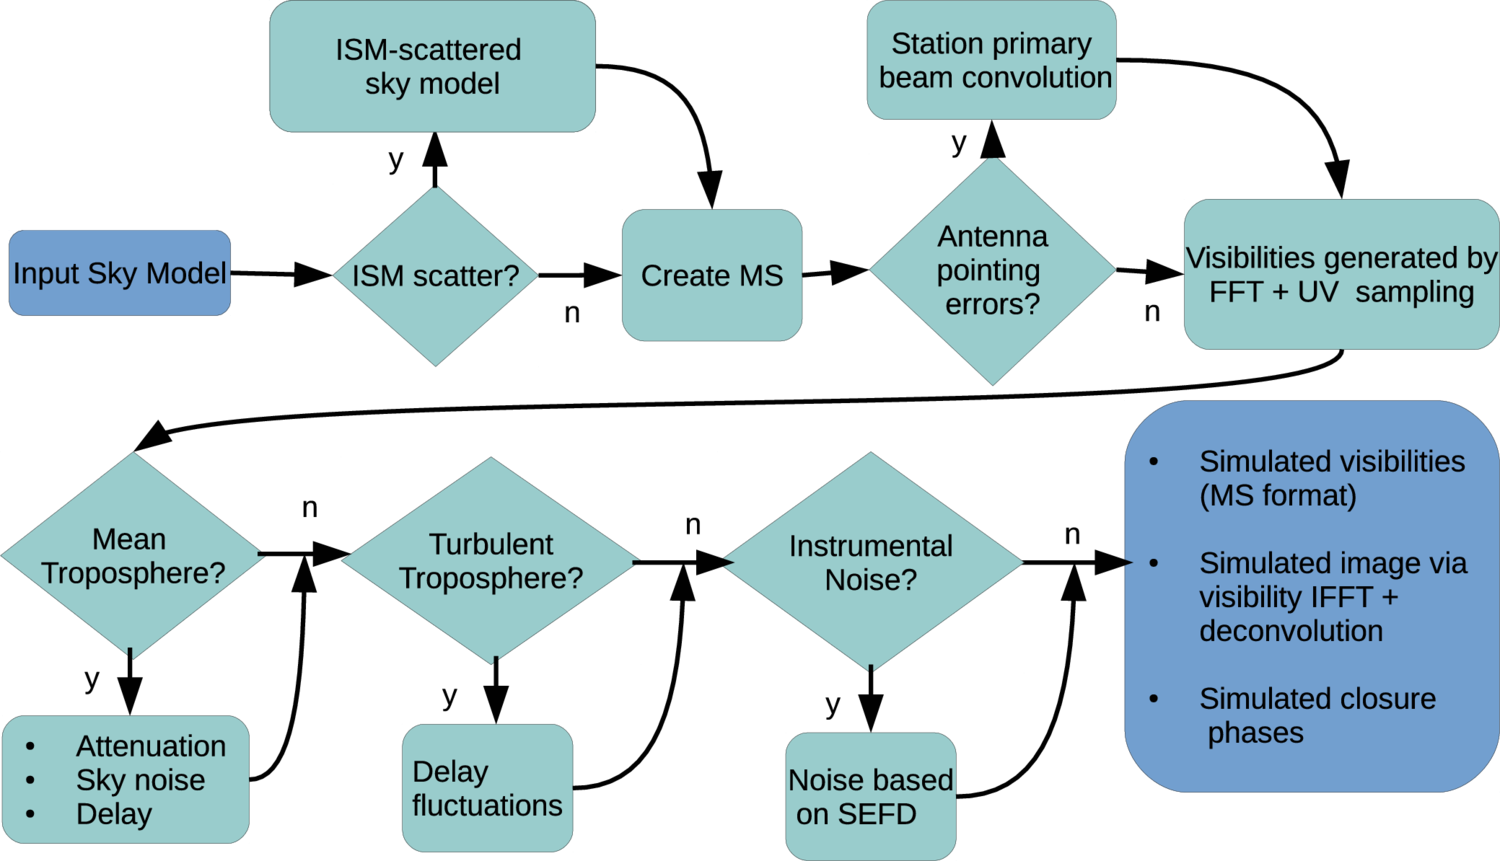
\includegraphics[width=1.4\columnwidth]{../../Images/flow_full}
\caption{Flow diagram showing basic sequence of the \textsc{MeqSilhouette} simulation pipeline. The sky model could include (a) a time-ordered list of {\sc fits} images or (b) parametric source model consisting of Gaussians or point sources. The details of the station information, observation strategy, tropospheric and ISM conditions are specified in a user-defined input configuration file. The pipeline is flexible, allowing any additional, arbitrary Jones matrices to be incorporated. Further details in text.\label{flow}%
}
\end{center}
\end{figure*}




\subsection{ScatterBrane}
%Pr 1 St 2


Scattering in the ISM at millimetre wavelengths falls into the strong scattering regime, which has been quantitatively described in the literature \citep*{Narayan_1989,Goodman_1989} and implemented in the \textsc{Python}-based \textsc{Scatterbrane}\footnote{http://krosenfeld.github.io/scatterbrane/current} package, based on \citet*{Johnson_2015a}. This approach extends the turbulent model described in section~\ref{sec:basic_scat} to regimes where the inner and outer turbulent scales as well as the anisotropy of scattering kernel are considered. The distance to the screen is taken from the best-fit solution from \citet{Bower_2013} and is located, not at the Galactic Centre, but rather in the Scutum spiral arm at a distance $D_{\rm os}=5.8 \pm 0.3$~kpc. 

The turbulent phase screen $\phi(\mathbf{x})$ is generated from the phase spatial power spectrum (see Appendix C \citet*{Johnson_2015a}) and the scattered image $I_{\rm ss}$ is approximated by 'reshuffling' of the source image $I_{\rm src}$
\begin{equation}
I_{\rm ss}(\mathbf{x}) \approx I_{\rm src}\left(\mathbf{x} + r_{\rm F}^2 \nabla \phi(\mathbf{x})\right),
\end{equation}
where $\nabla$ is the directional derivative. Even though $\phi(\mathbf{x})$ is only coherent to $\sim r_{\rm 0}$, $\nabla \phi(\mathbf{x})$ remains spatially coherent over much larger scales which results in the presence of large scale refractive substructure in the scattered image. 


We aim to place this description of ISM scattering, which has already yielded an important context for mm-VLBI observation \citep[e.g.][]{2016arXiv160106571O}, into a broader simulation framework. Our ISM module uses the public \textsc{Scatterbrane} code together with an interfacing task which ensures adequate time resolution for sampling ISM variability. If the time resolutions chosen to sample the source variability $\Delta t_{\rm src}$ and screen variability $\Delta t_{\rm ism}$ are unequal, we set  
\begin{itemize}
 \setlength\itemsep{1em}
\item $\Delta t_{\rm ism}=\Delta t_{\rm src}$ \qquad \qquad if \qquad  $\Delta t_{\rm src} < \Delta t_{\rm ism}$
\item $\Delta t_{\rm ism}=R(\frac{\Delta t_{\rm src}}{\Delta t_{\rm ism}})\Delta t_{\rm src}$ \ if \qquad  $\Delta t_{\rm src} > \Delta t_{\rm ism}$,
\end{itemize}
where $R$ rounds the fraction to the nearest integer. 

1. We are in the average image regime due to source size.
2. Code moves pixels arounds by ~ refractive scale ~10 uas..proportional to phase gradient 
3. The direction and magnitude of shuffling should be coherent to about ~ a few uas. (rf**2 * coherency of phase gradient)
4. Key assumption is that there is no source flux on baselines long enough to resolve the inner scale.(0.1 muas)
5. Averaging in bandwidth and time. Refractive noise is wideband..time variation over an hour ~ 0.5 uas. won't do much

\subsection{Atmospheric}
%Pr 1 St 2
make table using that cool online table maker\\

\subsection{Pointing}
%Pr 1 St 2

\subsection{RODRIGUES interface}
%Pr 3 St 3
For community use, we host the online, RODRIGUES, interface, found at http://rodrigues.meqtrees.net/. Each of the components of the simulator run in Docker containers. **Looks like the infrustructure is going to change, re: discussions with Gijs and Sphe, so going to wait before writing this.

\section{Parameter estimation}
%Leave for now
